\section{Validation}

\subsection{1D Analytical Retardation Benchmark}\label{sec:1D}

The 1D linear-retardation benchmark tests the surface-chemistry coupling on a
uniform domain where the retardation factor has an exact analytical form.
With uniform porosity $\theta$ and surface-area density $a_{\mathrm{surf}}$,
the field-level retardation coefficient is
$R_{\mathrm{field}} = 1 + a_{\mathrm{surf}} K_{s,\mathrm{field}} / \theta^2$,
and the retarded concentration front satisfies the standard advection--diffusion
equation with effective velocity $u / (\theta R_{\mathrm{field}})$ and effective
diffusivity $D / R_{\mathrm{field}}$.
This configuration therefore isolates three coupled components of the
implementation: the batch-secant calibration of $K_{s,\mathrm{field}}$, the
field-level averaging of the surface-capacity term, and the advective--diffusive
transport step. The benchmark compares a surface-enabled transport case, a
matched aqueous-only case (\mbox{$a_{\mathrm{surf}} = 0$}), and a dilute batch
pair used to estimate $K_{s,\mathrm{field}}$ via the secant method.

For the validated benchmark reported here,
$K_{s,\mathrm{field}} = 4.241 \times 10^{-6}$ and
$R_{\mathrm{field}} = 2.696$, so the surface-enabled front travels at
$1/R_{\mathrm{field}} \approx 37\%$ of the aqueous-only front velocity.
The mesh contains $80 \times 1 \times 1$ cells and uses a species diffusion
coefficient of $10^{-11}\ \mathrm{m^2\,s^{-1}}$.
The surface-enabled profile matches the retarded advection--diffusion reference
with a relative L1 error of $1.43\%$ and $L_{\infty}$ error of $3.67\%$.
The aqueous-only profile matches its unretarded reference with L1 and
$L_{\infty}$ errors of $1.08\%$ and $5.97\%$, respectively.
The field-level total-equivalent inventory---the domain integral of the combined
aqueous and adsorbed mass---differs from the analytical limit by $1.57\%$ for
the surface-enabled run and by $0.58\%$ for the aqueous-only run.

The solver therefore reproduces the dilute field-level retardation limit of the
DBS formulation with bulk inventory error below $1.6\%$. Because the domain
geometry is uniform, any residual error reflects inaccuracies in the
surface-chemistry coupling and the batch-secant estimation procedure rather than
mesh or geometry artefacts. Figure~\ref{fig:1DRetardation} shows the spatial
profiles at $t = 10$, and Figure~\ref{fig:1DBreakthrough} shows the
outlet breakthrough curves over the full run to $t = 80$~s.
The surface-enabled breakthrough arrives at $1/R_{\mathrm{field}} \approx 37\%$
of the aqueous-only breakthrough time, in agreement with the analytical prediction.
The classical semi-infinite Ogata--Banks solution~\citep{ogata1961solution} is also
shown for comparison and predicts systematically later breakthrough: because the
simulation uses a Neumann (no-flux) outlet, solute cannot diffuse past $x = L$
and accumulates there faster than the semi-infinite formula assumes.
The finite-domain reference, which solves the same 1-D advection--diffusion
equation on $[0, L]$ with a Dirichlet inlet and Neumann outlet matching the
OpenFOAM boundary conditions exactly, captures this effect and gives the
agreement shown.

\begin{figure}[htbp]
    \centering
    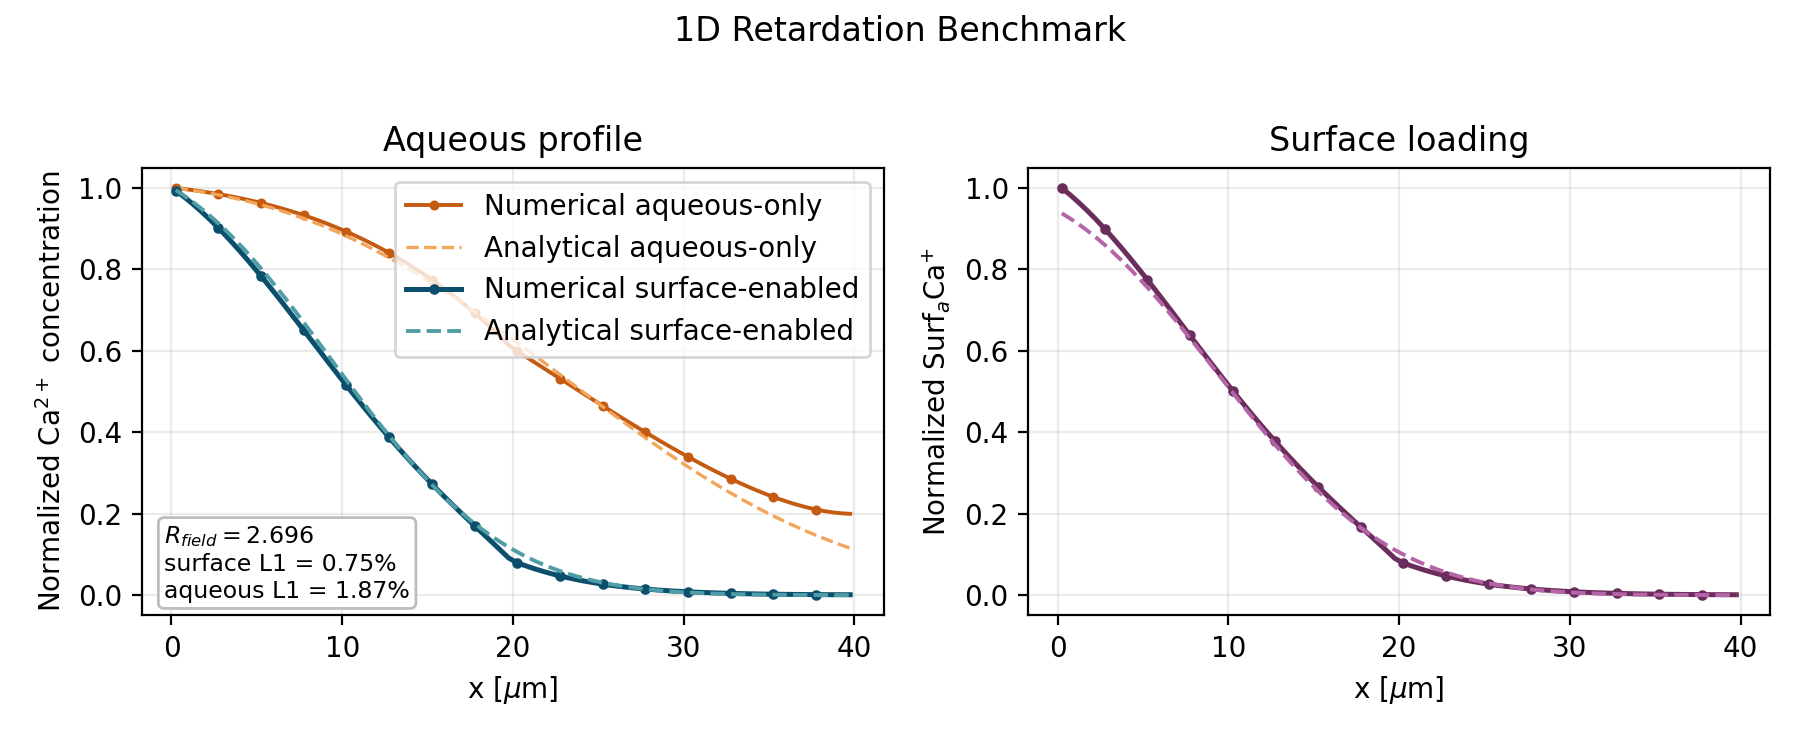
\includegraphics[width=0.9\linewidth]{figures/png/fig01_1d_retardation.png}
    \caption{1D analytical retardation benchmark: spatial profiles at $t = 10$.
    Left: normalized aqueous Ca$^{2+}$ profiles for the aqueous-only and
    surface-enabled runs, compared against their matching cell-averaged
    advection-diffusion analytical solutions. Right: normalized surface loading
    compared against the cell-averaged linear-equilibrium analytical limit
    constructed from the calibrated field-level $K_{s,\mathrm{field}}$.}
    \label{fig:1DRetardation}
\end{figure}

\begin{figure}[htbp]
    \centering
    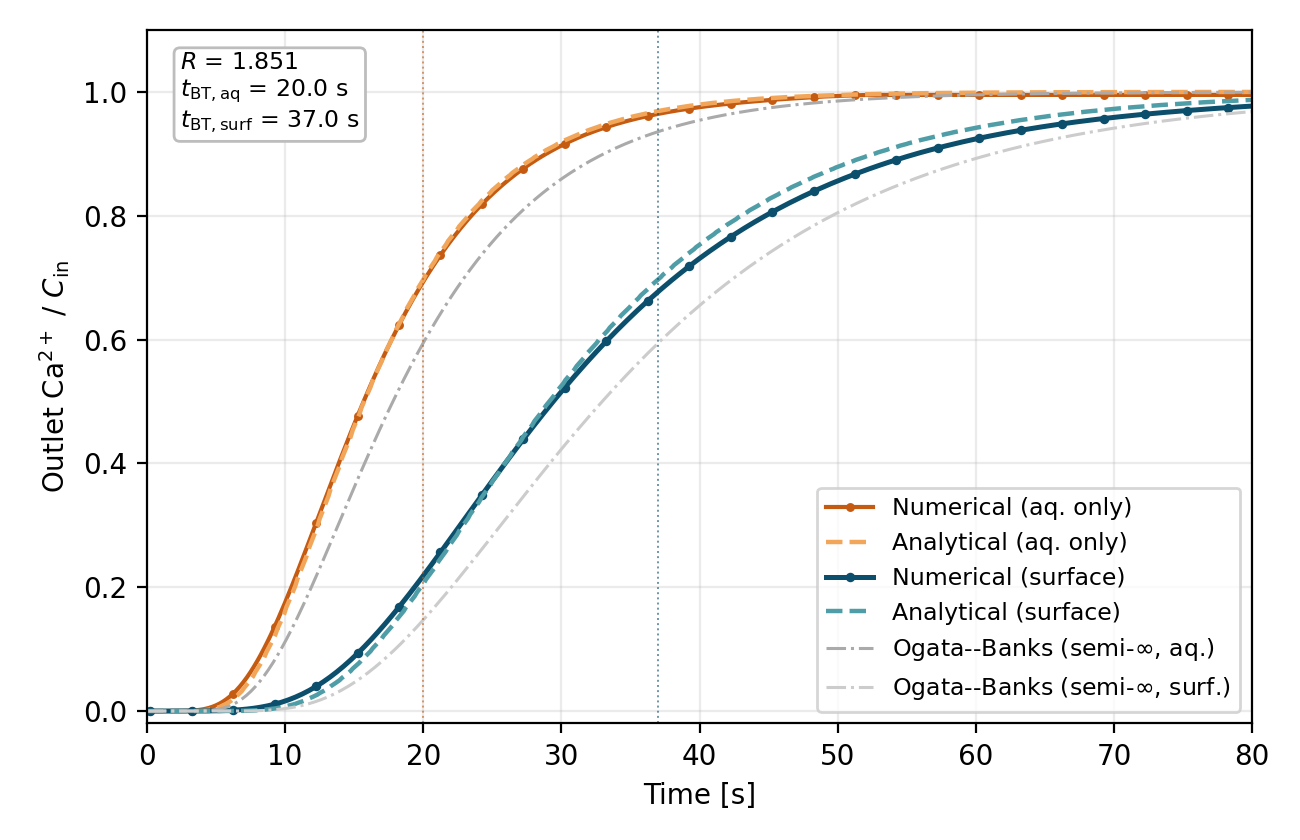
\includegraphics[width=0.9\linewidth]{figures/png/fig06_1d_breakthrough.png}
    \caption{1D outlet breakthrough curves. Symbols show the outlet-patch
    area-averaged Ca$^{2+}$ normalised by the inlet concentration $C_{\mathrm{in}}$
    for the aqueous-only run (circles) and the surface-enabled run (squares).
    Dashed lines are the finite-domain analytical reference; dash-dot lines are
    the semi-infinite Ogata--Banks solution~\citep{ogata1961solution}.
    Vertical dotted lines mark the advective breakthrough times
    $t_{\mathrm{BT}} = L\theta/U$ (aqueous-only) and
    $t_{\mathrm{BT}} = L\theta R_{\mathrm{field}}/U$ (surface-enabled).}
    \label{fig:1DBreakthrough}
\end{figure}

\subsection{Closed-System Batch Balance}

The chemistry--transport interface is verified against the exact
species-inventory identity for a closed batch domain (no inflow or outflow,
$\mathbf{u} = 0$).
Conservation of the total field-level Ca$^{2+}$ inventory requires
\begin{equation}
    \mathcal{M} \;=\; \theta\,C + a_{\mathrm{surf}}\,\Gamma \;=\; \mathrm{const},
    \label{eq:closedBalance}
\end{equation}
where $C$ is the aqueous concentration, $\Gamma$ is the surface loading, and
$\theta$ and $a_{\mathrm{surf}}$ are the same domain-averaged porosity and
surface-area density as in the 1D transport benchmark.
In the linear dilute limit, Eq.~\eqref{eq:closedBalance} gives the equilibrium
partition
\begin{equation}
    C_{\mathrm{eq}} = \frac{\theta\,C_0}{\theta + a_{\mathrm{surf}}\,K_{s,\mathrm{field}}},
    \label{eq:batchEquil}
\end{equation}
which is equivalent to $C_0 / (1 + a_{\mathrm{surf}}\,K_{s,\mathrm{field}}/\theta)$.

Two tests are run on the 80\,\texttimes\,1\,\texttimes\,1 mesh with
$\theta = 0.5$ and $a_{\mathrm{surf}} = 10^5\,\mathrm{m^{-1}}$ using the same
Ca$^{2+}$--\texttt{Surf\_a} surface chemistry as in Section~\ref{sec:1D}.
In the \emph{adsorption} test the domain is initialised with a fully aqueous
inventory ($\theta\,C_0 = 4.49 \times 10^{-4}\,\mathrm{mol\,m^{-3}}$,
$\Gamma_0 \approx 0$) and the batch-equilibration solver brings the system to
equilibrium in a single PHREEQC call; Ca$^{2+}$ partitions from the pore
fluid onto the surface.
In the \emph{desorption} test the inventory is loaded entirely onto the
surface ($\Gamma_0 > 0$, $C_0 \approx 0$) and equilibrium is re-established;
Ca$^{2+}$ desorbs back into the pore fluid.
The relative inventory drift
$|\mathcal{M}_{\mathrm{end}} - \mathcal{M}_{\mathrm{start}}| / \mathcal{M}_{\mathrm{start}}$
is $1.2 \times 10^{-7}$ for adsorption and $7.2 \times 10^{-7}$ for
desorption, both well below the \mbox{$10^{-6}$} tolerance.
This confirms that the chemistry--transport interface conserves the total
field-level Ca$^{2+}$ inventory to the PHREEQC convergence level in both
the adsorption and desorption directions.

\subsection{Validation Summary}\label{sec:valSummary}

In addition to the 1D analytical benchmark and the closed-system batch
balance, the solver has been verified against a set of controlled numerical
baselines on the same domain.
The aqueous-only and \mbox{$a_{\mathrm{surf}} = 0$} reductions confirm that
the solver degrades correctly to standard advection--diffusion transport when
surface chemistry is absent.
Closed-system adsorption--desorption cycles confirm that the total
aqueous-plus-surface Ca$^{2+}$ inventory is conserved at relative drifts of
$1.2 \times 10^{-7}$ and $7.2 \times 10^{-7}$, demonstrating that the
chemistry--transport interface preserves global species balance to the
PHREEQC convergence level in both directions.
Sensitivity studies on the operator-splitting step size, the physical
timestep, and the mesh resolution quantify the local and bulk drift at
practical settings.
Table~\ref{tab:validationSummary} summarises the key metrics from this
benchmark family.

\begin{table}[htbp]
    \centering
    \caption{Validation summary for the tracked 1D benchmark family.
    ``Splitting'' refers to the operator-splitting (chemistry--transport)
    consistency test; ``Timestep'' and ``Mesh'' are sensitivity studies on
    the fixed 1D benchmark. The performance row reports the fraction of
    wall-clock time spent in PHREEQC across the sensitivity runs.}
    \label{tab:validationSummary}
    \begin{tabular}{lll}
        \toprule
        Check & Metric & Result \\
        \midrule
        Analytical 1D & Surface L1 / total drift & $1.43\%$ / $1.57\%$ \\
        Closed-system (ads./des.) & Inventory drift & $1.2\times10^{-7}$ / $7.2\times10^{-7}$ \\
        Splitting     & Local / bulk drift        & $3$--$4.5\%$ / $<0.6\%$ \\
        Timestep      & Local / bulk drift        & $\approx 3\%$ / $0.25\%$ \\
        Mesh          & Front / total drift       & $2.5\times 10^{-7}$ / $0.37\%$ \\
        Performance   & Surface chemistry fraction & $36$--$55\%$ \\
        \bottomrule
    \end{tabular}
\end{table}

A consistent pattern emerges across the sensitivity studies: local
(cell-level) drift reaches $3$--$4.5\%$ while bulk (volume-integrated) drift
stays below $0.6\%$.
This disparity indicates that operator-splitting and timestep errors are
concentrated near the chemical front and cancel almost completely at the domain
level, so global conservation properties are preserved even where local
truncation errors are non-negligible.
The near-zero front-position drift ($2.5 \times 10^{-7}$) from the mesh study
confirms that the retardation-front position is not systematically biased by
mesh resolution.
The surface chemistry fraction of $36$--$55\%$ of wall-clock time reflects the
per-cell cost of the PHREEQC equilibrium solve for a dilute two-ion system;
the same per-cell cost governs chemistry overhead in the 3D image-based cases,
where it scales with the number of mobile cells rather than with domain topology.

\subsection{Two-Scale Upscaling Validation}\label{sec:twoScaleValidation}

The upscaled formulation is tested directly against a fully resolved
lithium-sorption calculation on the same long micromodel geometry. The fully
resolved reference retains binary pore and grain cells, whereas the DBS case
represents the unresolved pore structure through its coarse-cell properties and
internal reactive surface area. Both cases use the same inlet chemistry and are
compared at matched P\'{e}clet number and normalized advective distance $x/L$.
This removes the difference in physical travel time caused by the separately
calibrated flow fields.

The fully resolved production resolution was selected after categorical
downsampling tests at $5$, $10$, and $15~\mu$m. Categorical majority voting was
used throughout: no pore/grain cell was formed by averaging to an intermediate
porosity. The $5~\mu$m image was retained because it preserves the streamwise
pore connectivity and the pore--grain interfaces on which sorption occurs;
coarser images gave increasing local Li-field differences even where bulk
porosity, permeability, and reactive area remained similar.

Figure~\ref{fig:twoScaleErrorPe} compares aqueous and sorbed Li at
$x/L=0.125$ for $\mathrm{Pe}=0.1$, $1$, $3$, and $10$. The acceptance limits
were $5\%$ absolute inventory difference, $10\%$ normalized streamwise-profile
L1 error, and $0.1$ map dissimilarity. Across the sweep, the largest aqueous
and sorbed inventory differences are $2.15\%$ and $1.83\%$, respectively; the
largest profile errors are $2.09\%$ and $5.19\%$; and every map dissimilarity
is below $8.0\times10^{-4}$. All four cases therefore pass the predefined
criteria. The error does not grow systematically with P\'{e}clet number, and no
breakdown of the upscaling is observed by $\mathrm{Pe}=10$ for this geometry.

\begin{figure}[htbp]
    \centering
    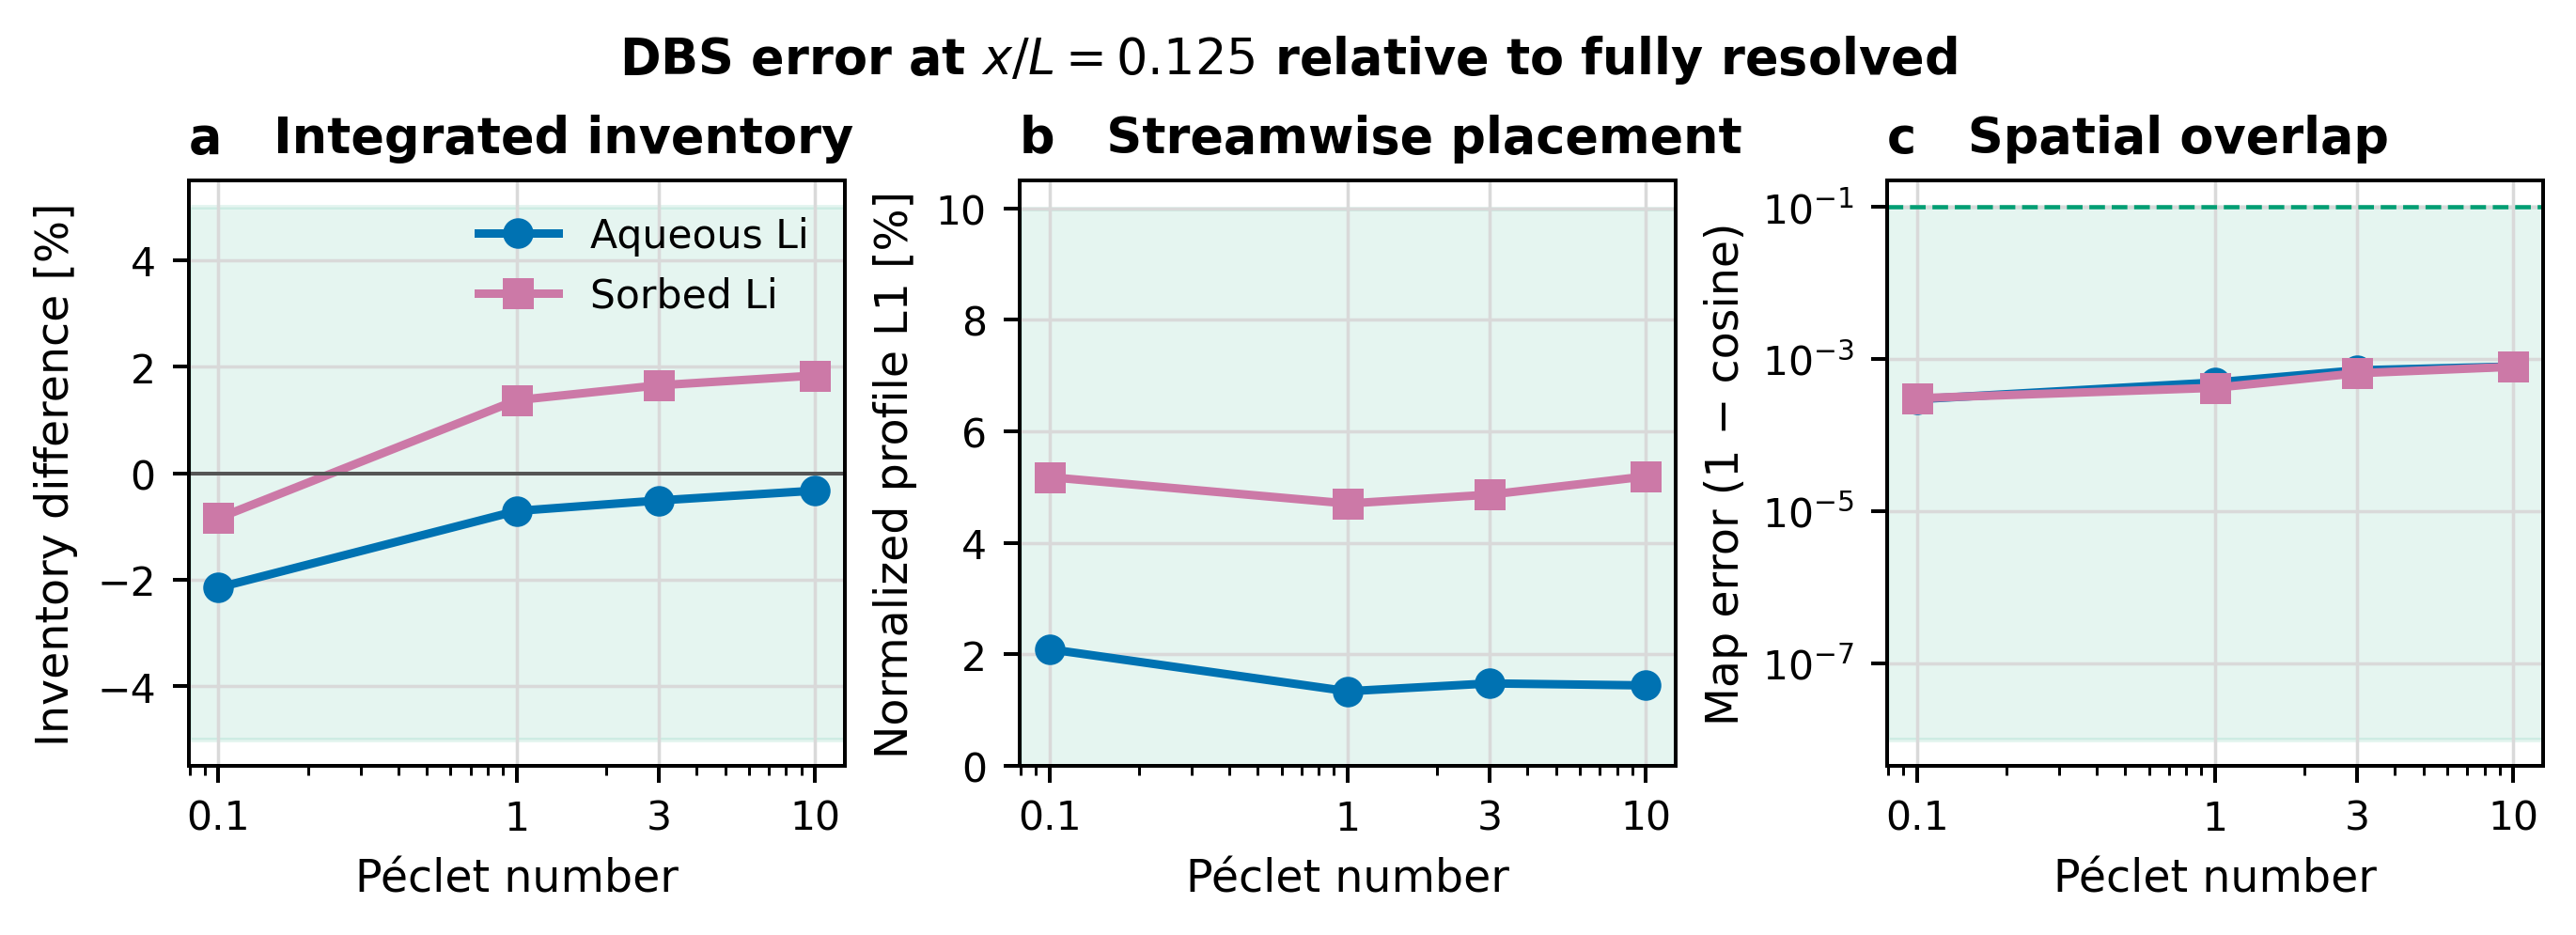
\includegraphics[width=\linewidth]{figures/png/fig09_two_scale_error_vs_peclet.png}
    \caption{DBS-upscaled error relative to the fully resolved lithium-sorption
    reference at matched $x/L=0.125$. (a)~Signed differences in integrated
    aqueous and sorbed Li inventory. (b)~Normalized L1 errors of the
    streamwise profiles. (c)~Map dissimilarity, defined as one minus cosine
    similarity. Green shading marks the predefined acceptance region in each
    panel.}
    \label{fig:twoScaleErrorPe}
\end{figure}

Figure~\ref{fig:twoScalePe1Fields} shows the fields later in the Pe=1 run, at
$x/L=0.625$. The resolved result is plotted on its native $5~\mu$m grid with
grain cells masked rather than spatially averaged. The pore-scale aqueous plume
and sorbed-Li pattern remain visible, while the DBS fields show the corresponding
coarse representation. Their front positions and large-scale plume shapes are
consistent despite the deliberately different local descriptions.

\begin{figure}[htbp]
    \centering
    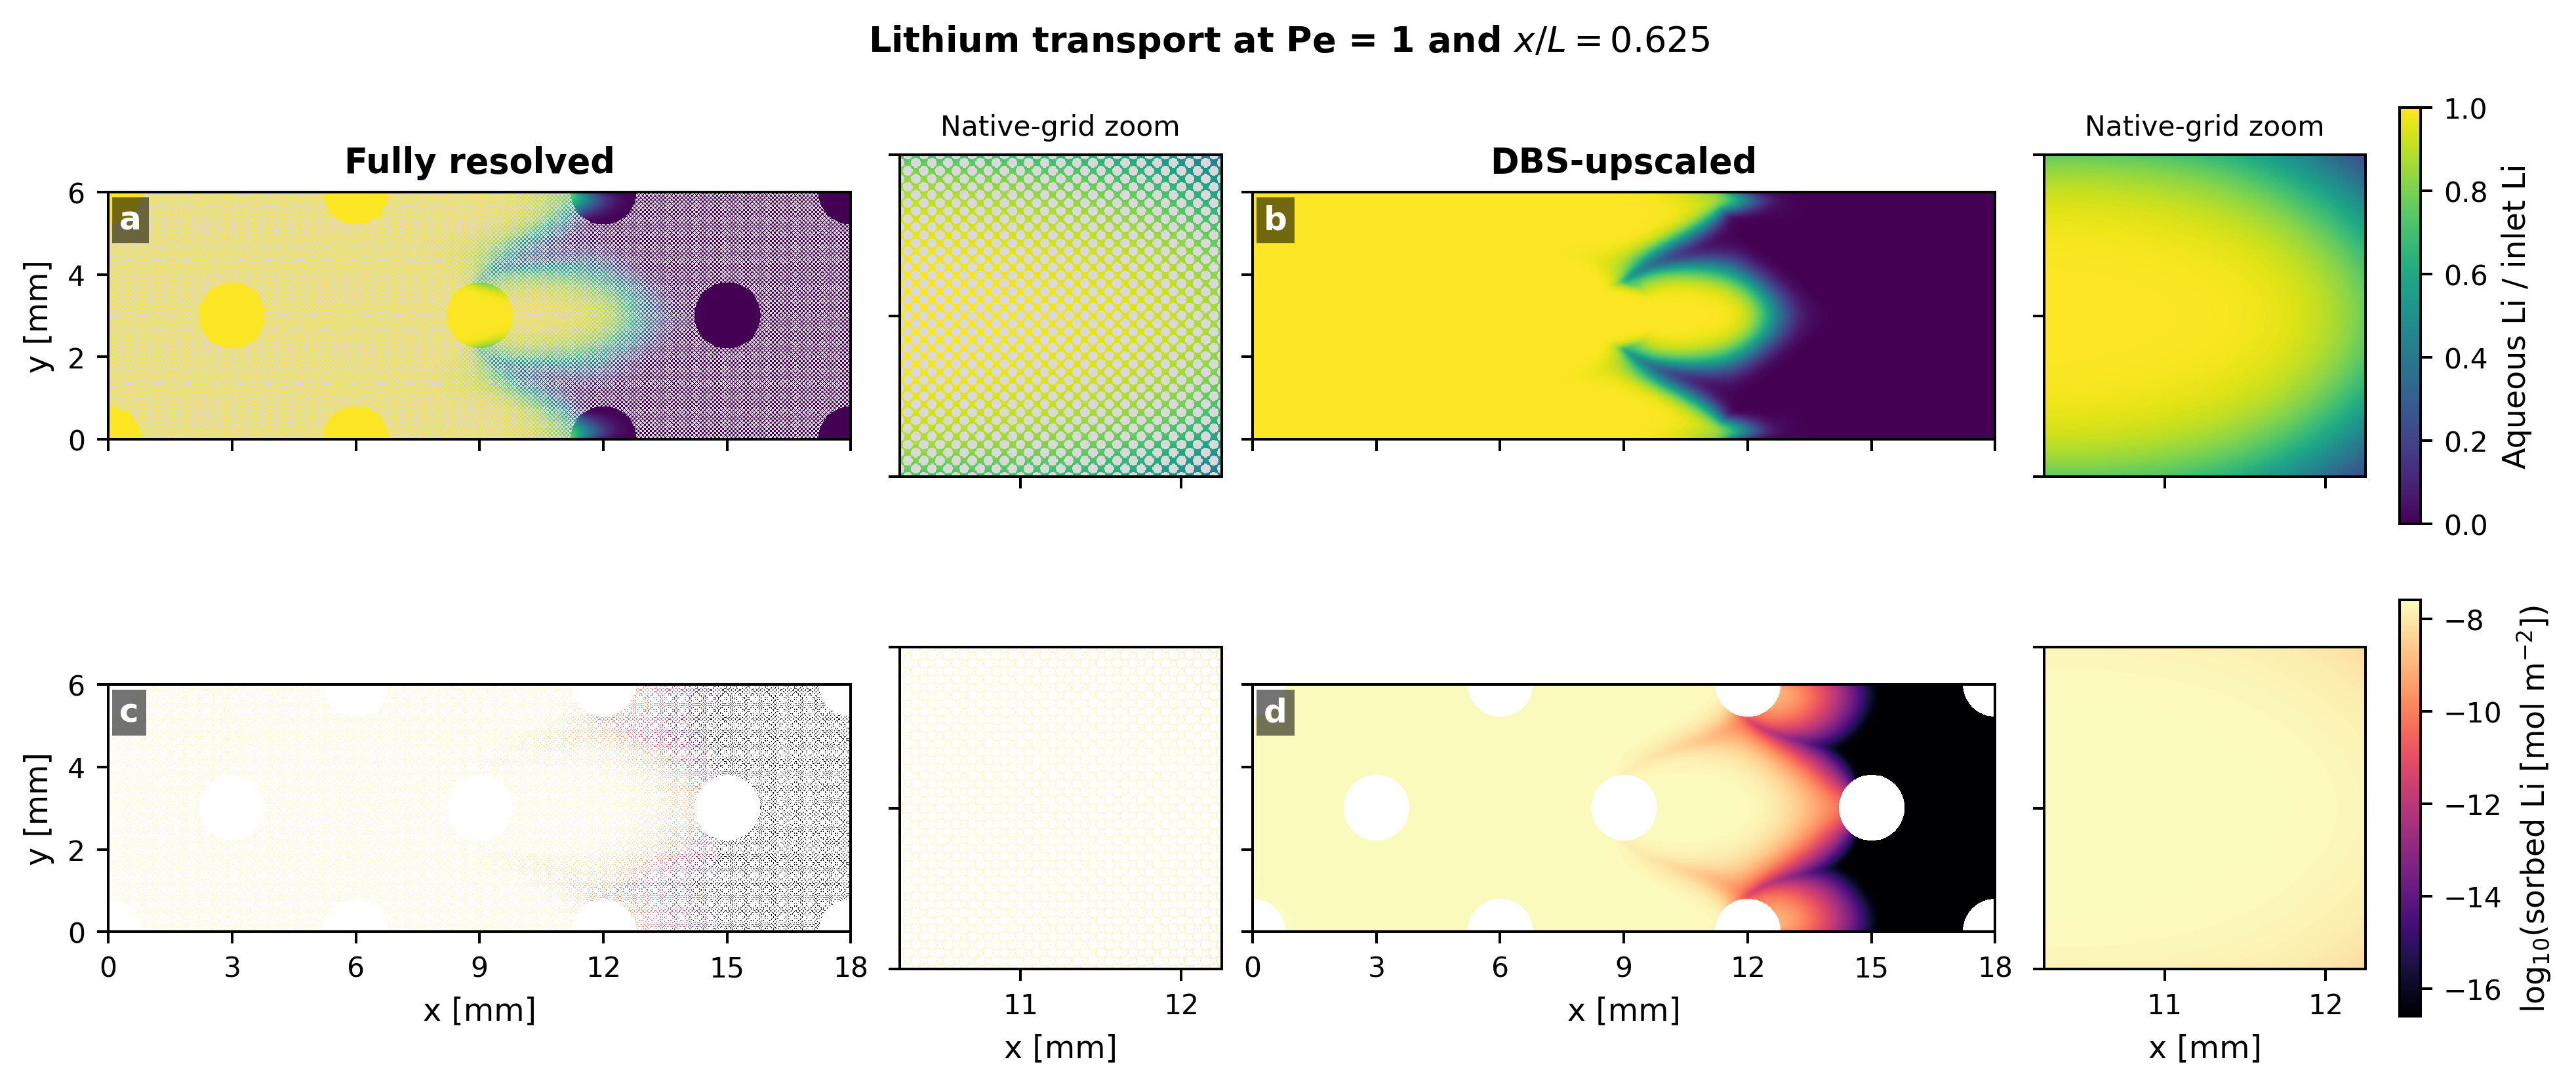
\includegraphics[width=\linewidth]{figures/png/fig10_two_scale_pe1_fields.png}
    \caption{Lithium fields at $\mathrm{Pe}=1$ and matched $x/L=0.625$.
    (a,b)~Aqueous Li normalized by the inlet concentration for the fully
    resolved and DBS-upscaled cases. (c,d)~Corresponding sorbed Li on a shared
    logarithmic scale. The inset panels show the native computational grids;
    the fully resolved pore/grain image is masked, not averaged.}
    \label{fig:twoScalePe1Fields}
\end{figure}
